%%=============================================================================
%% Methodologie
%%=============================================================================

\chapter{\IfLanguageName{dutch}{Methodologie}{Methodology}}
\label{ch:methodologie}

%% TODO: Hoe ben je te werk gegaan? Verdeel je onderzoek in grote fasen, en
%% licht in elke fase toe welke stappen je gevolgd hebt. Verantwoord waarom je
%% op deze manier te werk gegaan bent. Je moet kunnen aantonen dat je de best
%% mogelijke manier toegepast hebt om een antwoord te vinden op de
%% onderzoeksvraag.

In dit gedeelte van de bachelorproef wordt onderzocht of AI klaar is om Sentiment Analysis toe te passen in het bedrijfsleven. Er zullen een aantal mogelijkheden worden getest om te zien welke tool het meest nauwkeurig is. Zoals eerder vermeld, zal Sentiment Analysis klaar zijn om te gebruiken in het bedrijfsleven bij een succespercentage van 80 \%. 

De eerste tool die getest wordt is de Microsoft Azure Text Analytics API. 

\section{Microsoft Azure Text Analytics API}

\subsection{Achtergrond informatie}
\label{achtergrondinformatieazure}
Zoals eerder besproken, biedt Microsoft Azure SaaS-tools aan in de vorm van software. De Text Analytics API biedt dus ook NLP features aan voor text mining, text analysis, sentiment analysis, opinion mining,... \autocite{Microsoft2020} Deze API maakt deel uit van de Azure Cognitive Services. Deze biedt een volledig aanbod aan machine learning en AI algoritmes. Om deze services te gebruiken , moet de gebruiker wel een account aanmaken. \autocite{Microsoft2020}

Om deze Microsoft Text Analytics API te implementeren zal er gebruik gemaakt worden van Microsoft Visual Studio. Dit is een IDE (Integrated Development Environment) en wordt gebruikt om applicaties, websites en software te ontwikkelen voor Windows. Voor deze bachelorproef wordt de code in Microsoft Visual Studio geschreven, met name in de programmeertaal C\#. 

\subsection{Aanpak}
\label{aanpakazure}
\textbf{Stap 1}: De Text Analytics Resource

Om te beginnen moet er een Text Analytics Resource gemaakt worden in Azure zoals te zien op figuur 3.1. Een Text Analytics Resource is een service waardoor de gebruiker teksten kan analyseren zonder daarvoor de AI te moeten trainen. \autocite{Microsoft2020}

\begin{figure}[!htbp]
    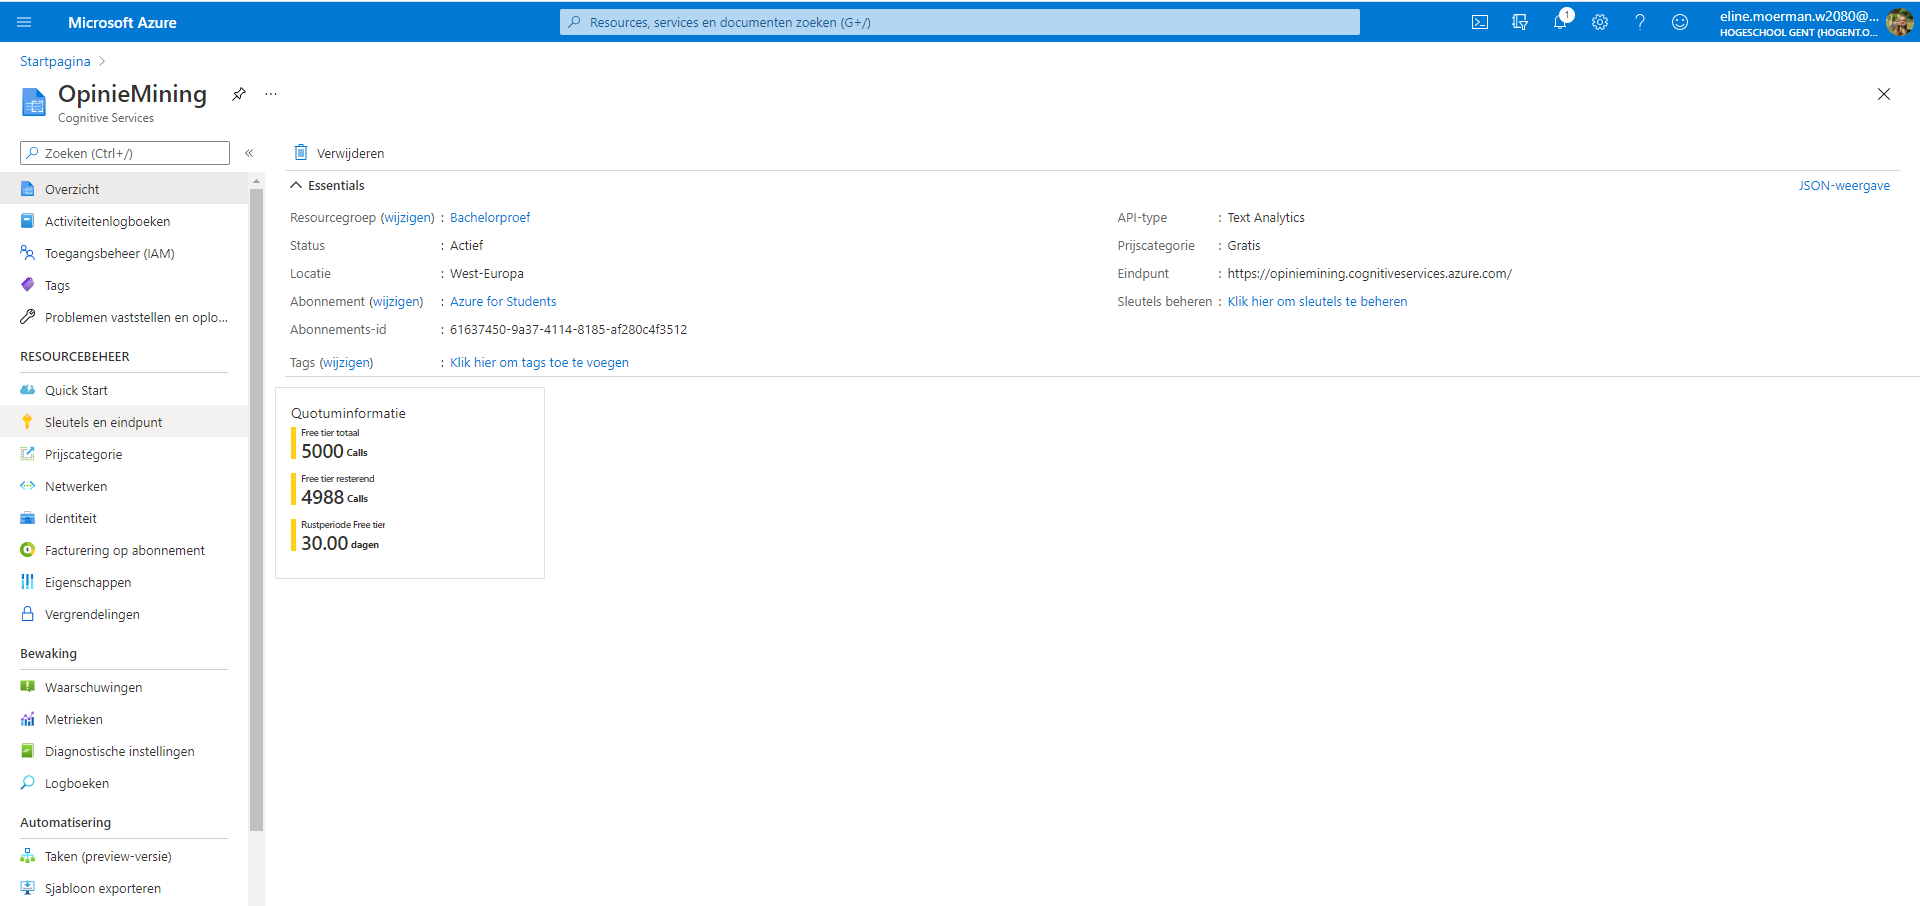
\includegraphics[width=\textwidth]{AzureResource.PNG}
    \caption{\label{azureresource}De Azure Text Analytics Resource \autocite{Microsoft2021}.}
\end{figure}
\FloatBarrier

Eenmaal de service aangemaakt is, genereert Azure een sleutel en een endpoint. Deze zullen gebruikt worden in Visual Studio om de Azure service te kunnen gebruiken. De key en endpoint zijn nodig zodat niemand anders van deze service kan gebruik maken. 

\textbf{Stap 2}: Een project opzetten in Visual Studio en de juiste packages installeren

Wanneer Visual Studio opgestart wordt, vraagt de applicatie om een nieuw project te maken. Hier is de beste keuze een .NET Core console applicatie. Dit zorgt ervoor dat er geen overbodige bestanden worden aangemaakt en dat enkel de klasse Program.cs aangemaakt zal worden. In deze file zal al de code geschreven worden om de datasets te kunnen analyseren. \autocite{Microsoft2020}

Daarna moet er een package geïnstalleerd worden. Een package is herbruikbare code die al door andere developers geschreven is en die de gebruiker kan downloaden in zijn of haar project. \autocite{Microsoft2018} De package die nodig is, is Azure.AI.TextAnalytics, zoals te zien op figuur 3.2.

\begin{figure}[!htbp]
    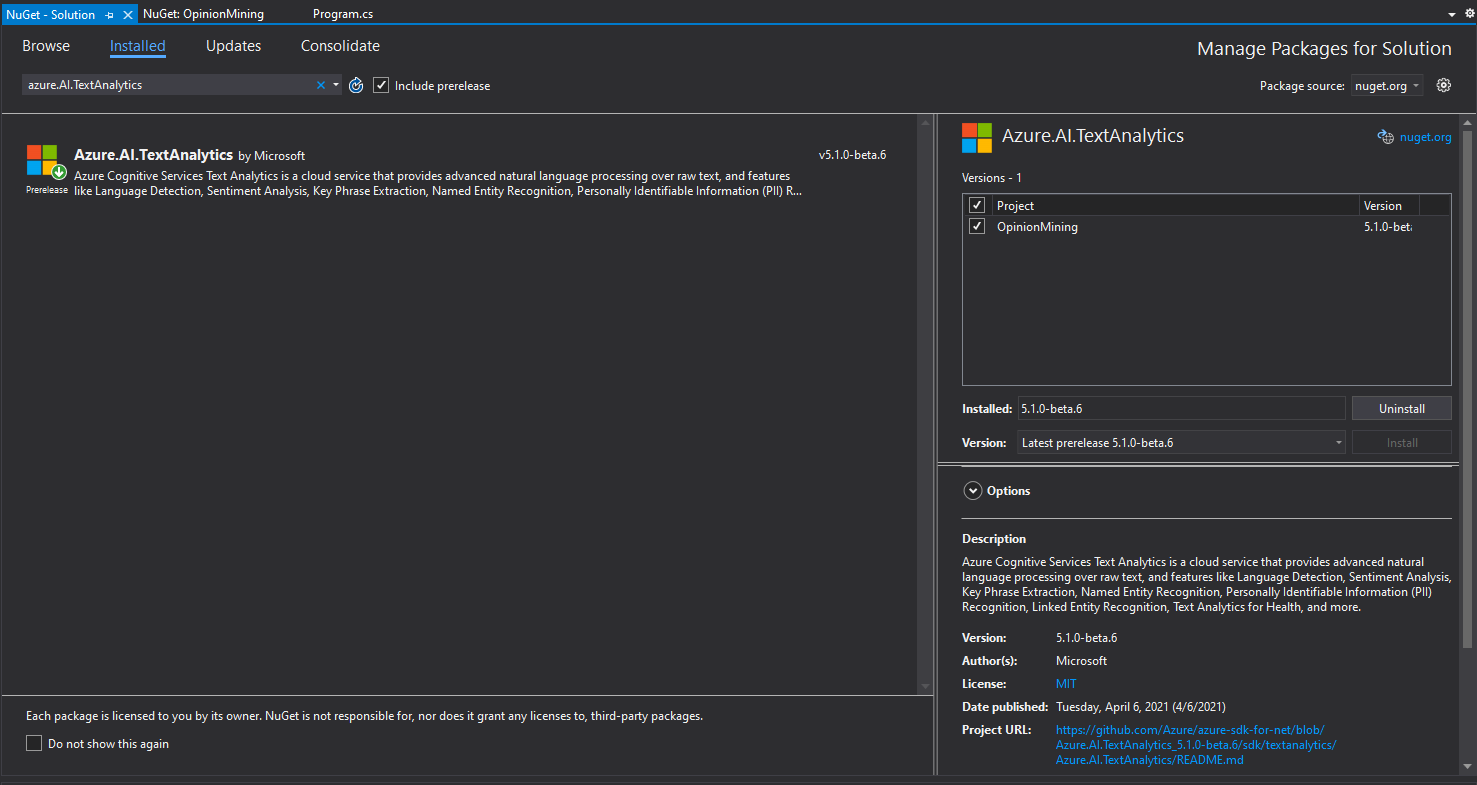
\includegraphics[width=\textwidth]{AzurePackage.PNG}
    \caption{\label{azurepackage}De Azure TextAnalytics Package \autocite{Microsoft2020}.}
\end{figure}
\FloatBarrier


\textbf{Stap 3}: De data omzetten naar het juiste formaat

Om de data uit de datasets te gebruiken, moet deze toegevoegd worden in Visual Studio. Allereerst wordt er een nieuwe klasse 'Data' aangemaakt. Hier zal alle data opgeslagen worden zodat deze later kan gebruikt worden. Daarna wordt er een een nieuw Google Colab document aangemaakt. Een Google Colab document is een tool waar de gebruiker code in Python kan schrijven. Dit gebeurt allemaal online, er moet geen software gedownload worden om deze tool te kunnen gebruiken. 

\textbf{Stap 4}: De juiste code schrijven om zinnen te kunnen analyseren

Met behulp van de Azure Text Analytics documentatie, kan de code in enkele methoden geschreven worden. Alle code wordt geschreven in de klasse Program.cs. 

\subsection{Amazon Dataset}
\label{amazondatasetazure}

\subsubsection{Data omzetten}
\label{amazondatasetomzettenazure}
Wanneer de Amazon dataset van het internet gehaald wordt, krijgt de gebruiker twee bz2 bestanden. Deze moeten natuurlijk omgezet worden zodat de data in Visual Studio geanalyseerd kan worden. Het is handig om de bestanden op Google Drive op te slaan aangezien men hier heel gemakkelijk vanuit een Google Colab document aankan. In figuur 3.3 wordt dit proces getoond. Om te beginnen, worden de juiste imports toegevoegd om data te kunnen analyseren. In dit bestand wordt er gebruik gemaakt van pandas, numpy en bz2. Daarna wordt er toegang tot Google Drive gemaakt. In een laatste stap worden de bestanden vanop Google Drive uitgelezen

\begin{figure}[!htbp]
    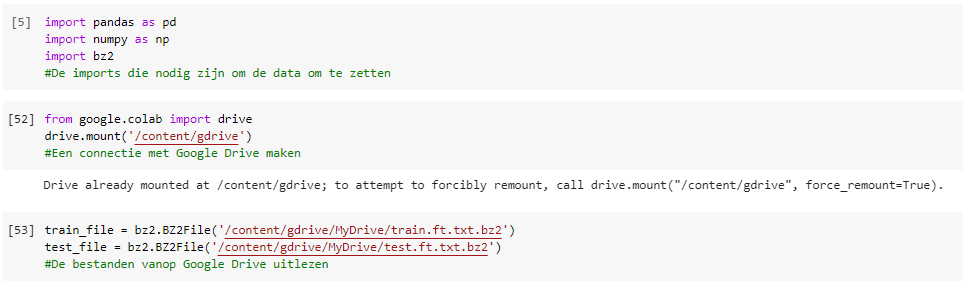
\includegraphics[width=\textwidth]{Stap1Omzetten.PNG}
    \caption{\label{stap1amazon}De bestanden worden opgehaald uit Google Drive.}
\end{figure}
\FloatBarrier

Daarna (figuur 3.4) wordt de data omgevormd tot bruikbare zinnen. Om te beginnen wordt de data via de functie readlines() omgezet naar een lijst van items waar elke lijn een object vormt. In het tweede blokje code wordt aangegeven hoe een review van de dataset eruitziet. Men kan zien dat er voor elke zin nog een b staat. Deze b moet weggefiltert worden, zodat de data naar tekst omgevormd wordt. 

Eenmaal dit gebeurd is, kan men in het vierde blokje code zien dat de b weg is.

\begin{figure}[!htbp]
    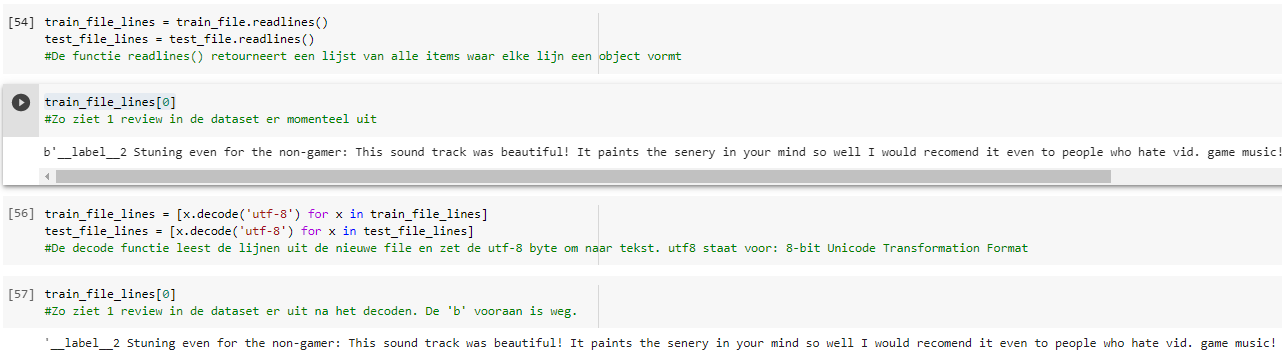
\includegraphics[width=\textwidth]{Stap2Omzetten.PNG}
    \caption{\label{stap2amazon}De data wordt omgezet naar tekst.}
\end{figure}
\FloatBarrier

Echter is dit nog niet genoeg om met deze data verder te werken. Vooraan elke zin staat ook nog een label. Dit label representeert een positieve of negatieve connotatie van de zin. Daarom worden de labels en de tekst opgeplitst in twee datasets, zoals te zien op figuur 3.5. De eerste dataset heet train\_labels: deze bevat de sentimenten die bij elke zin horen. Label1 wordt omgezet naar 0, label2 wordt omgezet naar 1. 1 representeert een positieve context, 0 een negatieve context. De tweede dataset heeft als naam train\_sentences: deze dataset bevat de eigenlijke zinnen die we door het programma in Visual Studio zullen laten lopen. In codeblokje twee staat een voorbeeld van hoe een zin er nu uit ziet, in codeblokje 3 staat een voorbeeld van hoe een score er nu uit ziet. 

\begin{figure}[!htbp]
    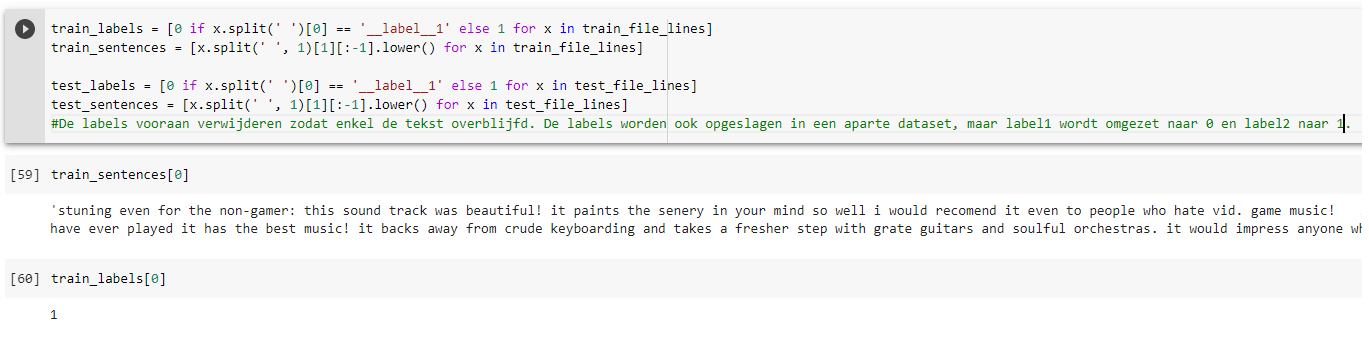
\includegraphics[width=\textwidth]{Stap3Omzetten.PNG}
    \caption{\label{stap3amazon}De data wordt opgeplitst.}
\end{figure}
\FloatBarrier

Verder zijn er veel url's die gebruikt worden in de zinnen. Deze zijn niet nodig om de connotatie van een zin te analyseren. Via onderstaande methode in figuur 3.6 worden de url's uit de tekst gefilterd.

\begin{figure}[!htbp]
    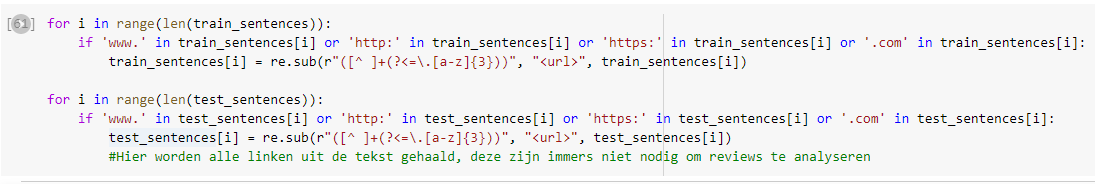
\includegraphics[width=\textwidth]{Stap4Omzetten.PNG}
    \caption{\label{stap4amazon}De url's worden uit de zinnen gehaald.}
\end{figure}
\FloatBarrier

Om te visualiseren hoe de data er momenteel uitziet, worden de zinnen in een dataframe geplaatst. Daarna worden de eerste 100 items getoond via de methode head(100).

\begin{figure}[!htbp]
    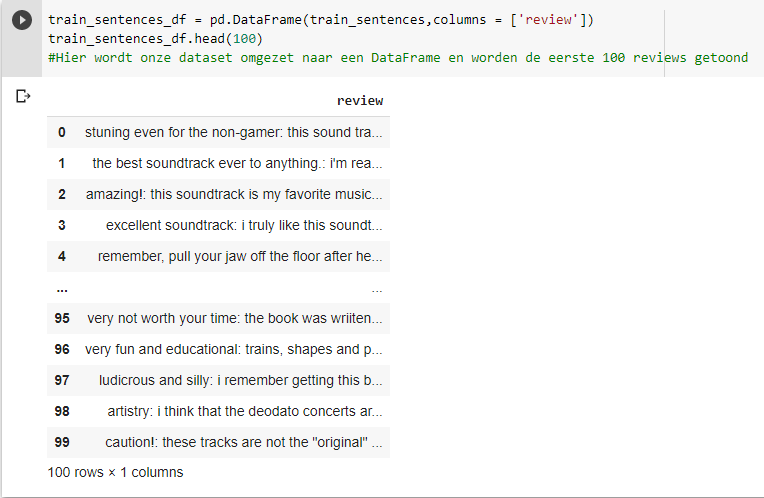
\includegraphics[width=\textwidth]{Stap5Omzetten.PNG}
    \caption{\label{stap5amazon}De data wordt omgezet naar een DataFrame.}
\end{figure}
\FloatBarrier

Zodat de zinnen gemakkelijk in Visual Studio kunnen toegevoegd worden, worden de eerste 500 zinnen met de methode head(500) geprint en wordt deze omgezet in de vorm Sentences.Add(zin). Zo kan dit gemakkelijk en zonder problemen gekopieerd worden naar Visual Studio.

\begin{figure}[!htbp]
    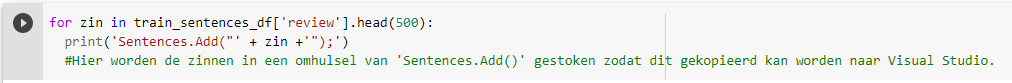
\includegraphics[width=\textwidth]{Stap6Omzetten.PNG}
    \caption{\label{stap6amazon}De zinnen worden in een formaat gegoten dat gemakkelijk in Visual Studio kan gebruikt worden.}
\end{figure}
\FloatBarrier

In figuur 3.9 kan men zien dat de zinnen die hiervoor gegenereerd werden, gekopieerd zijn naar de klasse Data. De zinnen worden in een lijst van strings gestopt die men 'Sentences' noemt. De scores worden in een lijst van ints gestoken, nadat deze omgezet zijn in figuur 3.10.

\begin{figure}[!htbp]
    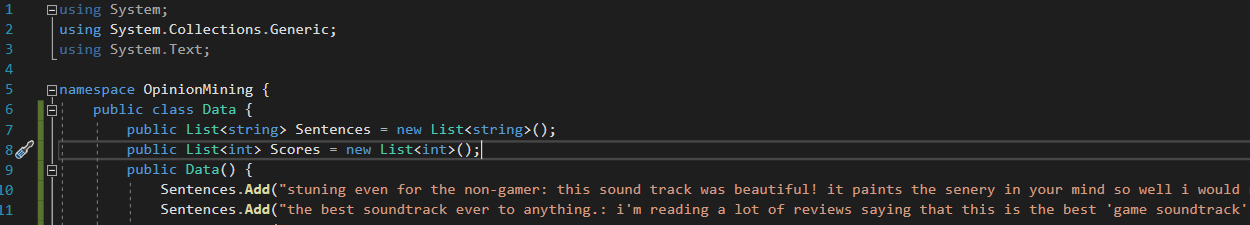
\includegraphics[width=\textwidth]{Stap7Omzetten.PNG}
    \caption{\label{stap7amazon}De zinnen worden toegevoegd in de klasse Data.}
\end{figure}
\FloatBarrier

\begin{figure}[!htbp]
    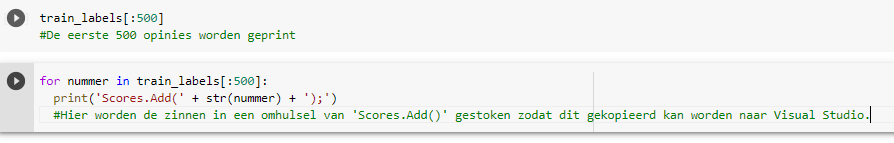
\includegraphics[width=\textwidth]{Stap8Omzetten.PNG}
    \caption{\label{stap8amazon}De scores worden in een formaat geplaatst dat gemakkelijk in Visual Studio kan gebruikt worden.}
\end{figure}
\FloatBarrier


\subsubsection{Visual Studio}
\label{amazondatasetvisualstudioazure}
Nu de data-omzetting gebeurd is, beschikt Visual Studio over een lijst van 500 zinnen met bijbehorende score. Een score 0 betekent dat de zin als 'negatief' beschouwd wordt, terwijl een score van 1 een positieve connotatie voorstelt. Om te kijken of de Azure Text Analytics API de zinnen ook werkelijk juist categoriseert, zal er een bepaalde nauwkeurigheid berekend moeten worden. 

Maar om dit te verwezenlijken, moet er eerst een connectie met de Azure Text Analytics resource gemaakt worden. Dit gebeurt aan de hand van de endpoint en de key. Deze worden bovenaan in de klasse Program.cs geplaatst. Alle code zal vanaf nu in deze klasse geschreven worden. 

\begin{figure}[!htbp]
    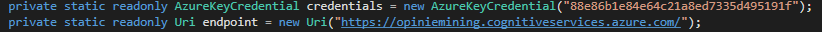
\includegraphics[width=\textwidth]{AzureKeyCredentials.PNG}
    \caption{\label{azurecredentials}De endpoint en key worden bovenaan de klasse geplaatst.}
\end{figure}
\FloatBarrier

Eenmaal de connectie in orde is, kan het onderzoek aan de slag gaan met de Azure Text Analytics API. Ten eerste zal er getest worden of de Azure resource alle zinnen ook daadwerkelijk herkent als 'Engels'. In sectie 2.3.1 wordt besproken wat Language Detection juist is. Deze techniek zal via een geschreven methode toegepast worden op alle zinnen. Als de getetecteerde zin gelijk is aan 'English', dan zal de nauwkeurigheid (in het codevoorbeeld: accuracy) verhoogd worden met 1. Als alle zinnen juist gezien worden als Engels, wordt er een nauwkeurigheid van 500/500 bereikt. 

\begin{figure}[!htbp]
    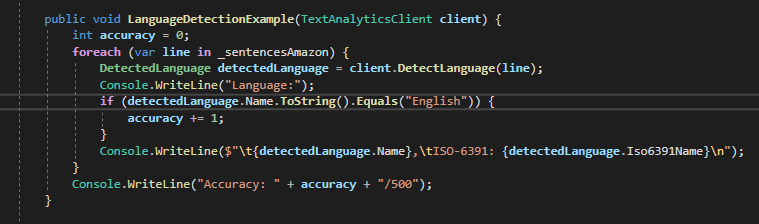
\includegraphics[width=\textwidth]{LanguageDetectionAmazon.PNG}
    \caption{\label{azurelanguagedetectionamazon}Language Detection in Visual Studio.}
\end{figure}
\FloatBarrier

Ten tweede zal er getest worden of de Azure Text Analytics API Sentiment Analysis juist kan toepassen. In sectie 2.4 wordt uitvoerig besproken wat Sentiment Analysis juist is. Via onderstaande methode in figuur 3.13 zal de nauwkeurigheid van de resource getest worden op 500. Bij deze methode is er echter nog wat toelichting nodig. De Azure Text Analytics API kan de zinnen categoriseren als Positief, Neutraal, Negatief en Gemengd. De Amazon dataset bevat enkel de informatie of een zin positief of negatief is. 

Daarom wordt er bij elke zin die juist positief of juist negatief bestempeld wordt, een punt bij de nauwkeurigheid opgeteld. Wanneer de zin als uitkomst Neutraal of Gemengd krijgt, wordt er per stukje tekst gekeken of dit positief of negatief is. Als er meer positieve stukjes zijn dan er negatieve stukjes zijn, wordt deze zin toch bestempeld als positief. Omgekeerd gebeurt hetzelfde voor negatief. 

\begin{figure}[!htbp]
    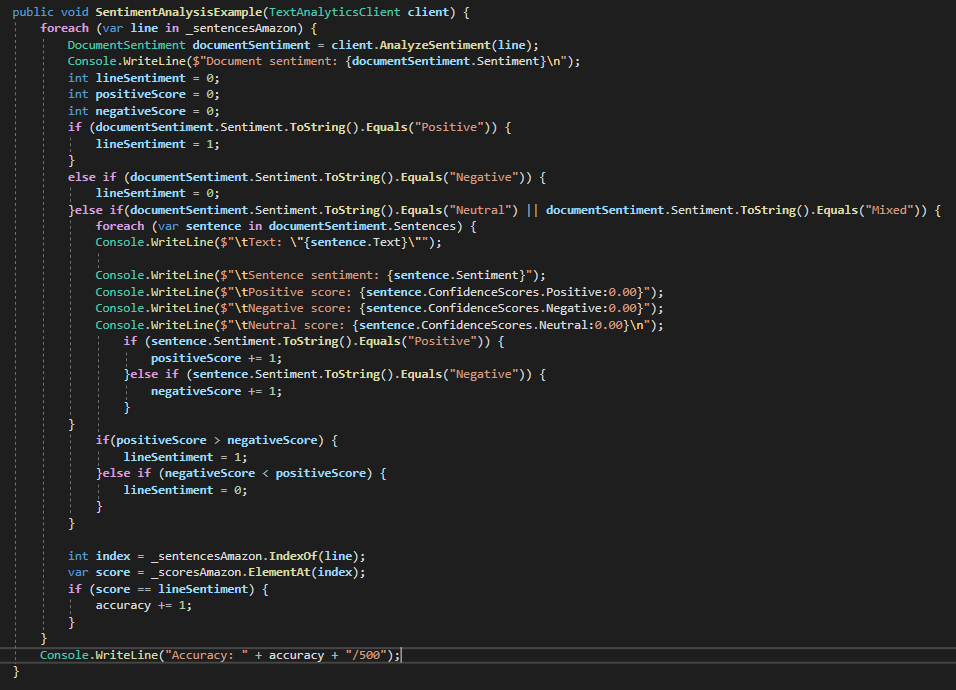
\includegraphics[width=\textwidth]{SentimentAnalysisAmazon.PNG}
    \caption{\label{azuresentimentanalysisamazon}Sentiment Analysis in Visual Studio.}
\end{figure}
\FloatBarrier

\subsubsection{Resultaten}
\label{amazondatasetresultatenazure}
Ten eerste werd er getest of de Azure Text Analytics API alle geselecteerde zinnen uit de dataset categoriseert als 'Engels'. In Figuur 3.14 ziet men dat de nauwkeurigheid 499/500 of 99.8\% is. Er werd 1 zin als 'Spaans' gecategoriseerd.

\begin{figure}[!htbp]
    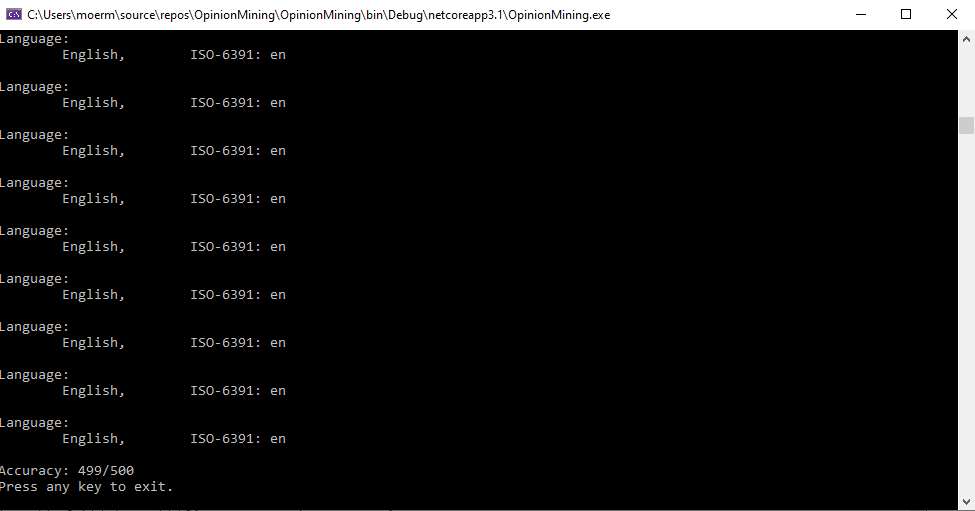
\includegraphics[width=\textwidth]{LanguageDetectionAmazonResult.PNG}
    \caption{\label{azurelanguagedetectionamazonresults}Language Detection voor de Amazon dataset in Visual Studio: Resultaten.}
\end{figure}
\FloatBarrier 

Ten tweede werd er getest of de Azure resource de zinnen uit de dataset juist kan categoriseren als positief of negatief. In figuur 3.15 kunnen de resultaten hiervan gevonden worden. De Azure Text Analytics API heeft 421/500 zinnen juist toegekend. Omgerekend is dit 84.2\%. In sectie 1.3 wordt er bepaald dat als een AI 80\% van de resultaten juist classifieert, dat deze als 'succesvol' kan gezien worden en dus bij bedrijven kan gebruikt worden. Voor deze dataset is dit dus zeker het geval, maar om te bepalen of dit betrouwbaar is, wordt dit ook getest op een tweede dataset, de Twitter Airlines dataset. 

\begin{figure}[!htbp]
    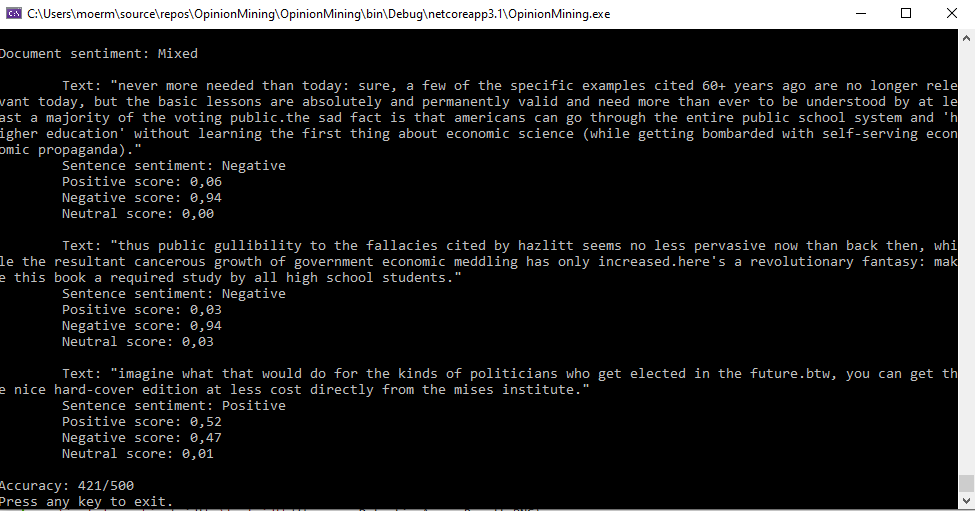
\includegraphics[width=\textwidth]{SentimentAnalysisAmazonResult.PNG}
    \caption{\label{azuresentimentanalysisamazonresults}Sentiment Analysis voor de Amazon dataset in Visual Studio: Resultaten.}
\end{figure}
\FloatBarrier 

\subsection{Twitter Airlines Dataset}
\label{twitterdatasetazure}

Ook bij de Twitter Airlines dataset worden dezelfde stappen gevolgd zoals eerder besproken in sectie 3.1.2 Aanpak. Ten eerste zal de data omgezet worden naar het juiste formaat, ten tweede zullen er enkele methodes uitgevoerd worden met deze data en ten slotte zullen de resultaten besproken worden. 

\subsubsection{Data omzetten}
\label{twitterdatasetomzettenazure}
Ook voor deze dataset moet de data omgevormd worden. Deze keer begint men met een csv bestand. een csv-bestand bevat 'comma separated values'. Met andere woorden wordt de data gescheiden door een komma. Om te beginnen importeren we juiste imports zoals numpy, pandas en re. Daarna moet er opnieuw verbinding gemaakt worden met Google Drive zodat het juiste csv bestand opgehaald kan worden. 
\begin{figure}[!htbp]
    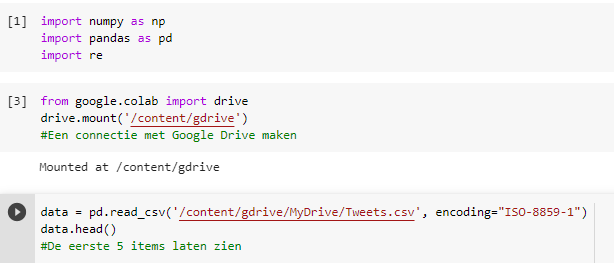
\includegraphics[width=\textwidth]{Stap1Twitter.PNG}
    \caption{\label{azurestap1twitter}Twitter Airline dataset: Imports afhandelen en connectie met Google Drive maken.}
\end{figure}
\FloatBarrier 

Daarna moeten de onnodige kolommen verwijderd worden, en dit zijn er heel wat. Enkel de scores en de zinnen zelf zijn nodig.
\begin{figure}[!htbp]
    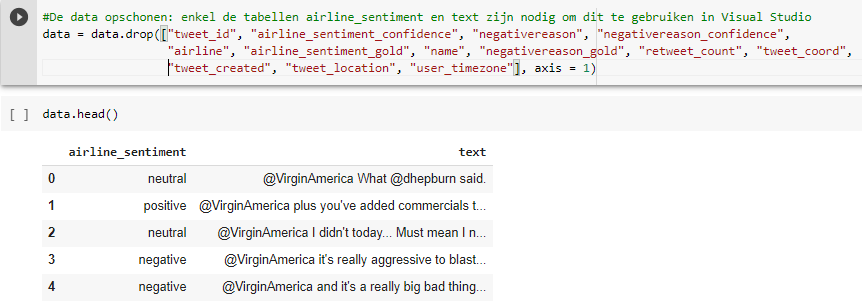
\includegraphics[width=\textwidth]{Stap2Twitter.PNG}
    \caption{\label{azurestap2twitter}Twitter Airline dataset: De onnodige kolommen verwijderen.}
\end{figure}
\FloatBarrier 

Hierna wordt de data opgeplitst. De zinnen worden in een variabele 'zinnen' geplaatst, terwijl de scores in een variabele 'sentiment' geplaatst worden. 
\begin{figure}[!htbp]
    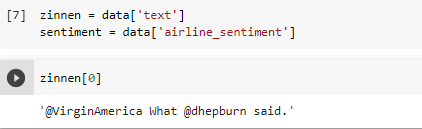
\includegraphics[width=\textwidth]{Stap3Twitter.PNG}
    \caption{\label{azurestap3twitter}Twitter Airline dataset: de score en de zinnen opsplitsen.}
\end{figure}
\FloatBarrier
Ten slotte worden de zinnen, zoals bij de Amazon dataset, in een nieuw formaat afgeprint zodat ze gemakkelijk te kopiëren zijn naar Visual Studio. 
\begin{figure}[!htbp]
    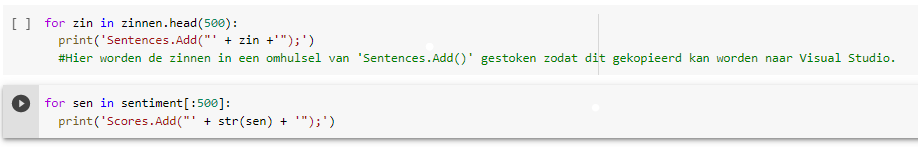
\includegraphics[width=\textwidth]{Stap4Twitter.PNG}
    \caption{\label{azurestap4twitter}Twitter Airline dataset: De zinnen en scores omzetten zodat ze in Visual Studio gebruikt kunnen worden.}
\end{figure}
\FloatBarrier 

\subsubsection{Visual Studio}
\label{twitterdatasetvisualstudioazure}
Voor deze dataset maken we gebruik van dezelfde endpoint en key als bij de vorige dataset, zoals te zien op figuur 3.11. Aan de methode voor gebruik te maken van Language Detection moet er in principe bijna niets aangepast worden. Enkel de dataset verandert. De methode die hier toegepast wordt, is ook te zien in figuur 3.12.

Ten tweede wordt ook hier getest of de Azure Text Analytics API de zinnen uit deze dataset kan categoriseren. Hiervoor moet de methode enigzinds aangepast worden aangezien de Twitter dataset wel neutrale connotatie herkent. In deze dataset worden de zinnen gezien als positief, negatief of neutraal. 

\begin{figure}[!htbp]
    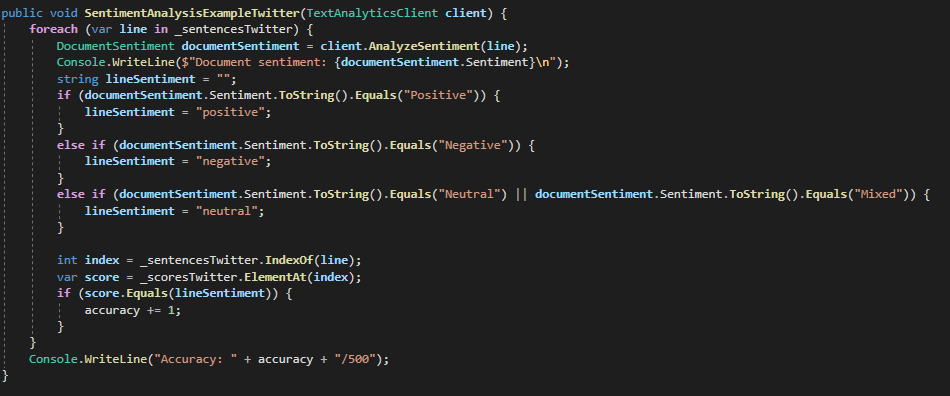
\includegraphics[width=\textwidth]{SentimentAnalysisTwitter.PNG}
    \caption{\label{azuresentimentanalysistwitter}Language Detection voor de Twitter dataset in Visual Studio: Resultaten.}
\end{figure}
\FloatBarrier 


\subsubsection{Resultaten}
\label{twitterdatasetresultatenazure}
Om te beginnen werd hetzelfde als bij de Amazon dataset getest, namelijk of alle zinnen als 'Engels' herkend worden. 
Hier haalt de Azure Text Analytics API een score van 499/500, omgerekend is dit 99.8\%. Één zin werd echter herkend als 'Frans'.

\begin{figure}[!htbp]
    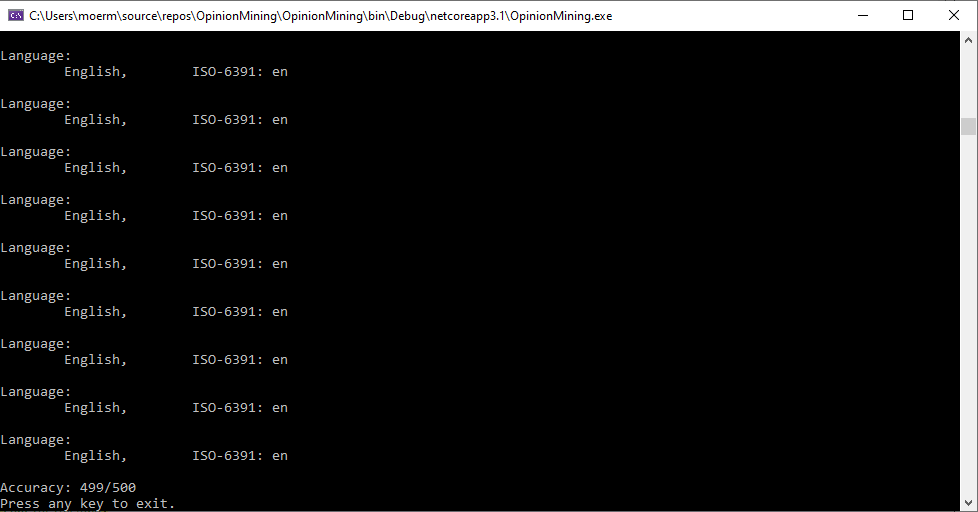
\includegraphics[width=\textwidth]{AccuracyTwitterDatasetAzure.PNG}
    \caption{\label{azurelanguagedetectiontwitterresults}Language Detection voor de Twitter dataset in Visual Studio: Resultaten.}
\end{figure}
\FloatBarrier 

Ten slotte werd er ook getest of Azure de zinnen juist herkent als positief, neutraal of negatief. In figuur 3.22 kunnen de resultaten hiervan terug gevonden worden. Er werd een score van 334/500 behaald door de Azure Text Analytics API. Omgerekend is dit 66.8\%. Dit is minder dan bij de Amazon dataset. Dit kan verklaard worden doordat 'tweets' korter zijn dan reviews, maar ook meer hashtags en apestaartjes bevatten. Verder worden er meer emoji's en tussentaal gebruikt bij tweets dan bij reviews.

\begin{figure}[!htbp]
    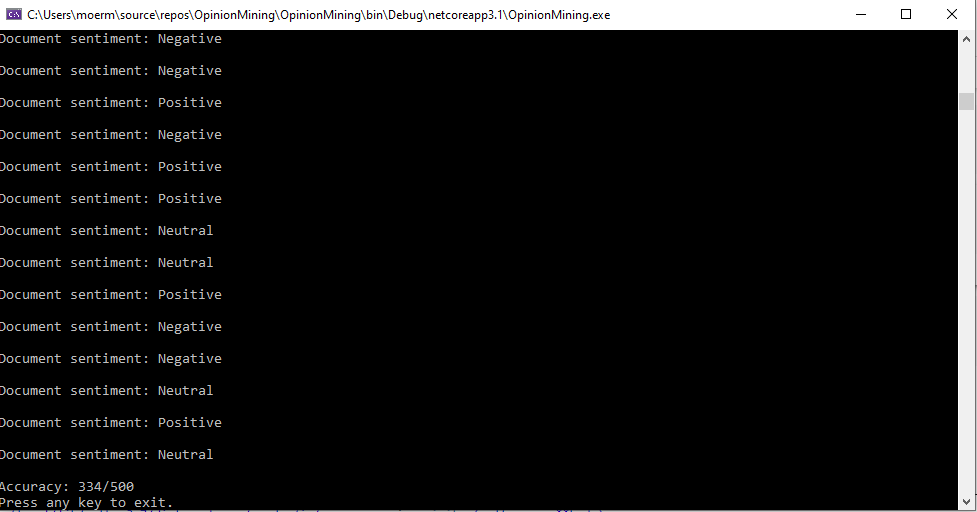
\includegraphics[width=\textwidth]{SentimentAnalysisTwitterResult.PNG}
    \caption{\label{azuresentimentanalysistwitterresults}Sentiment Analysis voor de Twitter dataset in Visual Studio: Resultaten.}
\end{figure}
\FloatBarrier 

\subsection{Conclusie Azure Text Analytics API}
\label{conclusieAzure}
De Azure Analytics API is heel goed voor Language Detection. Bij beide datasets behaalde de tool een score van 99.8\%. Voor Sentiment Analysis waren de resultaten verschillend bij beide datasets. De Amazon dataset had een nauwkeurigheid van 84.2\%, terwijl de Twitter dataset een score van 66.8\% behaalde. Dit is een enorm groot verschil en kan verklaard worden doordat tweets ten eerste meer tussentaal, emoji's, hashtags en apestaartjes bevatten dan reviews. Ten tweede speelt de lengte van de zinnen ook een belangrijke rol. Reviews zijn meestal langer dan tweets. De Azure Analytics API behaalt zo een gemiddelde score van 75.5\%, maar aangezien deze bachelorproef onderzoekt of Sentiment Analysis kan gebruikt worden bij reviews, is dit meer dan voldoende. 

\section{Google Cloud Platform}

Een tweede tool die getest wordt, is Google Cloud Platform. Ook hier zal de nauwkeurigheid van de tool berekend worden.

\subsection{Achtergrond informatie}
\label{achtergrondinformatiegooglecloudplatform}
Google Cloud Platform of GCP is een platform dat uiteraard aangeboden wordt door Google. Google Cloud Platform voorziet tools voor data-analyse, dataopslag en machine learning. \autocite{Bigelow2017}

Verder is Google Cloud Platform onderdeel van het bekende Google Cloud. Sinds 2011 biedt Google deze clouddienst aan, waardoor de gewone gebruiker gebruik kan maken van de producten die op dezelfde infrastructuur als Google draaien. \autocite{Bigelow2017}

Deze tool zal in de puntjes hieronder getest worden. 

\subsection{Aanpak}
\label{aanpakgoogleplatform}

De aanpak die hier toegepast wordt, kan ook teruggevonden worden in de developers guide van google. \autocite{Codelabs2021}

\textbf{Stap 1}: Setup

Om Google Cloud Platform te gebruiker, is er een account nodig. Daarom is de eerste stap om een account aan te maken. Het enige dat de gebruiker moet doen, is een visa-kaart voorzien. Hier wordt geen geld afgehaald, dit is enkel om te bewijzen dat de gebruiker geen robot is. 

Eenmaal het account aangemaakt is, komt men terecht op de homepagina van het platform. Het volgende dat nodig is, is een nieuw project. De verdere setup gebeurt via de Cloud Shell. Dit is een console dit gebruikt kan worden binnen het Google Cloud Platform. 

Met behulp van de Cloud Shell wordt de Natural Language API aan het project toegevoegd. 

\begin{figure}[!htbp]
    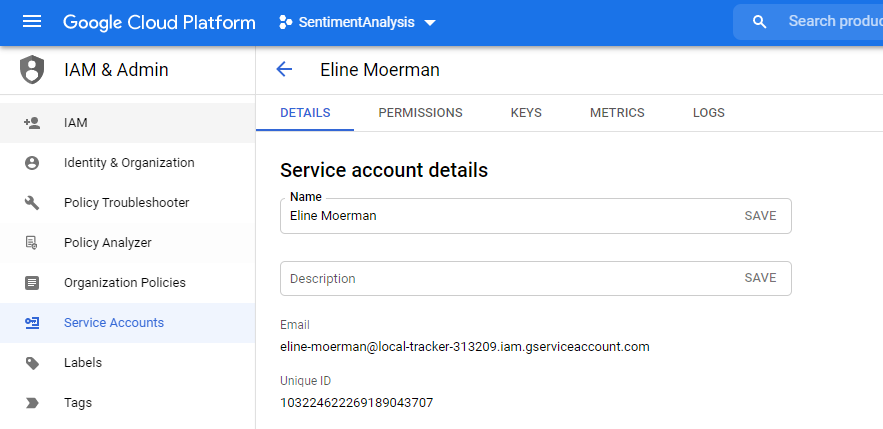
\includegraphics[width=\textwidth]{GoogleAccount.PNG}
    \caption{\label{googleaccount}De details van het nieuwe project.}
\end{figure}
\FloatBarrier 

\textbf{Stap 2}: Authenticatie

Om het platform te gebruiken, is er natuurlijk authenticatie nodig. Hiervoor moet er een 'key' gegenereerd worden. Dit gebeurt opnieuw via de Cloud Shell console. De commando's die hiervoor gebruikt worden, zijn te vinden in figuur 3.24.

\begin{figure}[!htbp]
    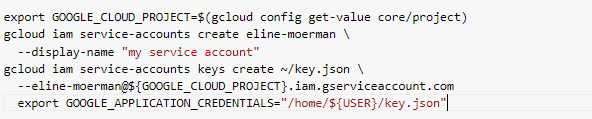
\includegraphics[width=\textwidth]{SetupGooglePlatform.PNG}
    \caption{\label{setupgoogleplatform}Een key genereren voor authenticatie.}
\end{figure}
\FloatBarrier 

\textbf{Stap 3}: Een C\# console applicatie opzetten

De laatste stap omvat het opzetten van een console applicatie. Via het commando 

dotnet new console -n \{Projectnaam\} 

wordt de applicatie aangemaakt. Hierna moet de Google Cloud Nuget package toegevoegd worden. Dit gebeurt via het commando

dotnet add package Google.Cloud.Language.V

Nadat alles opgezet is, kan de vereiste code geschreven worden.


\subsection{Amazon Datset}
\label{amazongoogleplatform}

De data werd op dezelfde manier omgezet als bij het testen van de Azure Text Analytics API. Deze omzetting kan gevonden worden van figuur 3.3 tot figuur 3.10.

\subsubsection{Code}
\label{amazoncodegoogleplatform}
De code wordt opnieuw geschreven in de klasse Program.cs. Google Cloud Platform werkt met een score die aan elke zin toegekend wordt. Een score tussen -1 en -0.25 betekent dat de tekst negatief is, een score tussen -0.25 en 0.25 betekent een neutrale score en een score tussen 0.25 en 1.0 staat voor een positieve connotatie. Aangezien de Amazon dataset enkel voorbeelden bevat die negatief of positief zijn, zijn de scores verdeeld als volgt: tussen -1 en 0 betekent negatief en tussen 0 en 1 betekent positief. In figuur 3.25 kan de geschreven code teruggevonden worden. Eenmaal alle data geanalyseerd is, komt er een nauwkeurigheid uit. 

\begin{figure}[!htbp]
    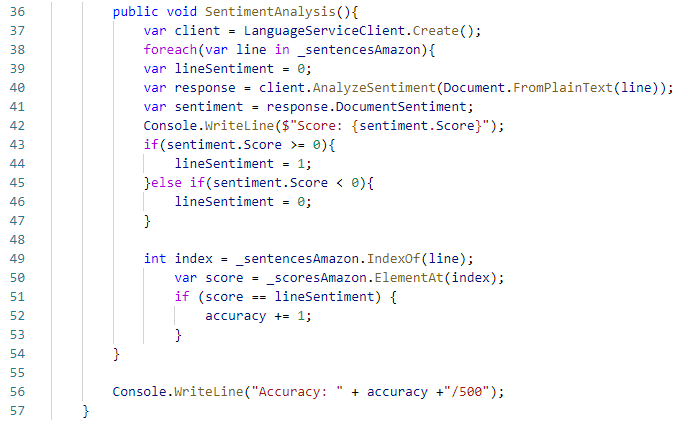
\includegraphics[width=\textwidth]{CodeAmazon.PNG}
    \caption{\label{codeamazon}Sentiment Analysis voor de Amazon dataset in Google Cloud Platform.}
\end{figure}
\FloatBarrier 

\subsubsection{Resultaten}
\label{amazonresultatengoogleplatform}

Er werd getest of Google Cloud Platform de zinnen uit de Amazon dataset juist kan categoriseren als positief of negatief. De resultaten hiervoor kunnen in figuur 3.26 teruggevonden worden. Na het analyseren van de zinnen, behaalde het platform een score van 465/500. Omgerekend is dit 93.0\%. Zoals eerder besproken, wordt een score van 80\% of hoger gezien als succesvol. Daarom kan geconcludeerd worden dat Google Coud Platform uitstekende resultaten biedt. Om meer zekerheid aan de lezer te bieden dat Google Cloud Platform een goede keuze is, wordt dit ook met de Twitter Airlines dataset getest. 
\begin{figure}[!htbp]
    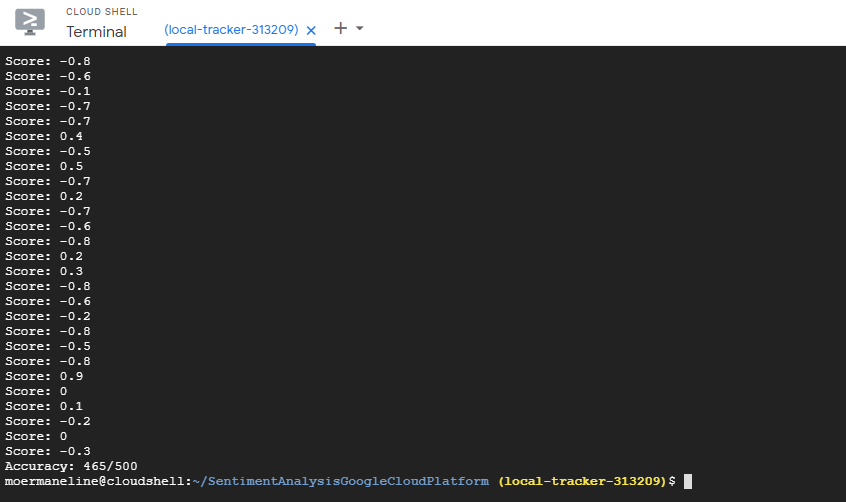
\includegraphics[width=\textwidth]{AccuracyAmazonGoogle.PNG}
    \caption{\label{accuracyTwitter}Google Cloud Platform resultaten voor de Amazon dataset.}
\end{figure}
\FloatBarrier 

\subsection{Twitter Airlines Datset}
\label{twittergoogleplatform}

De data werd op dezelfde manier omgezet als bij het testen van de Azure Text Analytics API. Deze omzetting kan gevonden worden van figuur 3.16 tot figuur 3.19.

\subsubsection{Code}
\label{twittercodegoogleplatform}
Aangezien de Twitte Airlines dataset wel data over de drie categorieën positief, neutraal en negatief bevat, kan Google Cloud Platform hier nauwkeuriger toegepast worden. Zinnen met een score boven de 0.25 krijgen een lineSentiment met waarde 'positief', zinnen met een score lager dan -0.25 krijgen een lineSentiment met waarde 'negatief' en zinnen met een score tussen de -0.25 en 0.25 krijgen 'neutraal'. Eenmaal alle zinnen door de code gegaan zijn, wordt er een nauwkeurigheid berekend op 500. De code kan teruggevonden worden in figuur 3.27.

\begin{figure}[!htbp]
    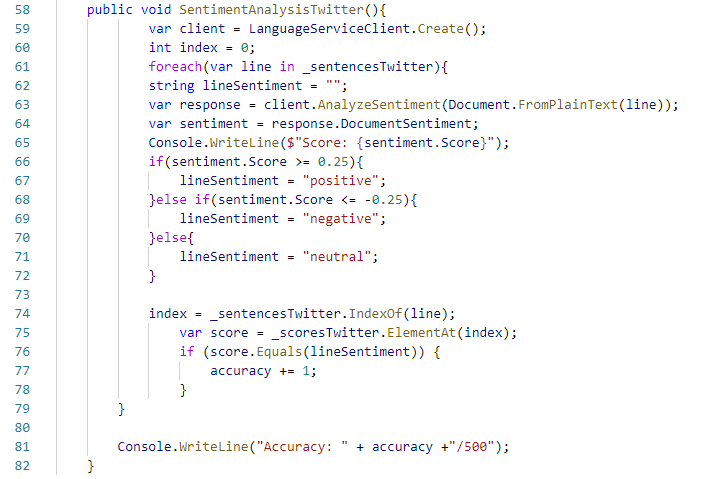
\includegraphics[width=\textwidth]{CodeTwitter.PNG}
    \caption{\label{codetwitter}Sentiment Analysis voor de Twitter dataset in Google Cloud Platform.}
\end{figure}
\FloatBarrier 

\subsubsection{Resultaten}
\label{twitterresultatengoogleplatform}
Er werd getest of Google Cloud Platform de zinnen uit de Twitter Airlines dataset ook juist kan categoriseren als positief, neutraal of negatief. De resultaten hiervoor kunnen in figuur 3.28 teruggevonden worden. Google Cloud Platform behaalde hier een score van 365/500. Omgerekend is dit 73.0\%. Zoals eerder besproken, wordt een score van 80\% of hoger gezien als succesvol. Daarom kan geconcludeerd worden dat Google Coud Platform redelijk goede resultaten biedt. Er werd eerder geconcludeerd dat de Twitter Airlines dataset steeds minder goede resultaten zal behalen omdat de tekst korter is, en de zinnen in een ander formaat staan. 

\begin{figure}[!htbp]
    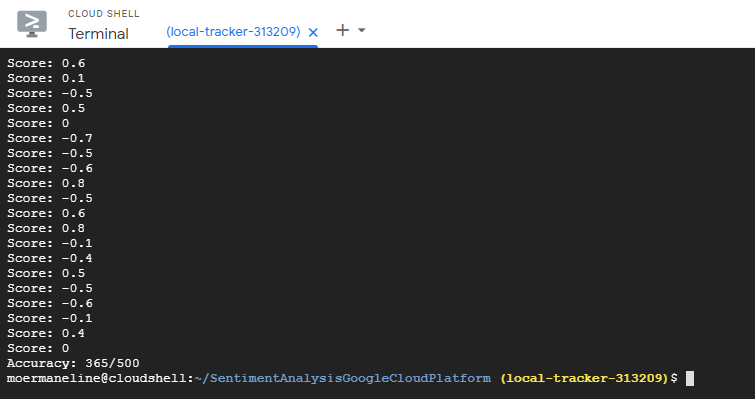
\includegraphics[width=\textwidth]{AccuracyTwitterGoogle.PNG}
    \caption{\label{accuracytwitter}Google Cloud Platform resultaten voor de Twitter dataset.}
\end{figure}
\FloatBarrier 

\subsection{Conclusie Google Cloud Platform}
\label{conclusieGoogleCloudPlatform}

Google Cloud Platform is goed voor Sentiment Analysis. De resultaten verschilden echter enorm tussen de twee datasets. De Amazon dataset had een nauwkeurigheid van 93.0\%, terwijl de Twitter dataset een score van 73.0\% behaalde. Dit verschil kan verklaard worden doordat tweets meer tussentaal, emoji's apenstaartjes en andere speciale tekens bevatten. Verder is de lengte van de zinnen in de Twitter dataset veel korter.Google Cloud Platform behaalt zo een gemiddelde score van 83.0\%, dit ligt mooi boven het gewenste 80\% succespercentage.


\section{Proof Of Concept}

In dit gedeelte wordt de data door eigen geschreven code getraind en wordt er geprobeerd om een betere of even goede nauwkeurigheid te behalen op de twee datasets als bij de Azure Text Analytics API. Het schrijven en testen van de code, gebeurt aan de hand van de stappen die in sectie 2.2.1 besproken werden. Data Preparatie is de eerste stap, daarna data cleaning gevolgd door het opzetten van de training en test dataset. In dit onderzoek zullen ook enkele visualisaties van de data gedaan worden om hier een beter begrip van te kunnen vormen. Ten slotte wordt het juiste model gekozen en getraind. 

\subsection{Data Preparatie}
\label{proofofconceptdatapreparatie}


